\chapter{研究背景和相关工作}
\label{cha:02_related_work}
本章的内容主要从两个方面对网络协议栈相关工作进行详细介绍,第一方面是在内核态直接对网络协议栈进行调优,第二方面是将网络协议栈搬离到用户态实现并进行更深度的优化。此外,对两种方式的优劣分别进行分析,并与本工作进行对比。

\section{内核态网络协议栈的优化工作}
\label{sec:02_kernel}

\subsection{Linux内核网络协议栈优化}
网络协议栈诞生初期就一直作为内核操作系统的一部分,毕竟数据包处理涉及到网卡硬件资源的管理,为了保证安全需要操作系统的内核态权限才能对硬件网卡直接进行操作。早在上个世纪八十年代,协议栈从内核分离出到用户态的想法就已经被提出~\cite{1987packer},但是由于在用户态进行数据包多路复用产生过多的上下文切换以及进程间通信的开销,所以当时的背景下在内核态实现实现协议栈有着更高的网络性能。

操作系统内核在不断演进中也为网络协议栈的优化做出不可磨灭的贡献。早期的TCP/IP协议栈存在着严重的多核扩展性问题,这主要因为多核共享资源的锁竞争造成的开销,如图\ref{fig:accept_queue_lock}所示,为了支持更多的并发,网络应用常常在多个核上开启多个并发流同时监听同一个listen socket,为了保证并发安全内核在共享的accept队列等全局资源中加入锁,这样在大量网络并发时候会造成严重的锁资源竞争开销,导致较差的多核扩展性,甚至造成随着CPU核数的提升,网络性能反而变得更差。

在内核中为了解决该问题,在Linux内核3.9版本中SO\_REUSEPORT~\cite{SO_REUSEPORT}选项被引入进来,该关键字使得不同socket可以绑定在同一个网络端口。如图\ref{fig:accept_queue_unlock}显示的是引进SO\_REUSEPORT后监听的工作模式,本质上就是将accept队列这个原来全局共享的资源拆分到每个核的每一个socket,减少锁资源的竞争开销。不过该功能需要应用程序在调用socket函数时候添加SO\_REUSEPORT作为参数,对用户并不透明,所以兼容性并不是好。

% \vspace{-10pt}
\begin{figure}[htbp]
\centering
\begin{minipage}[t]{0.48\textwidth}
\centering
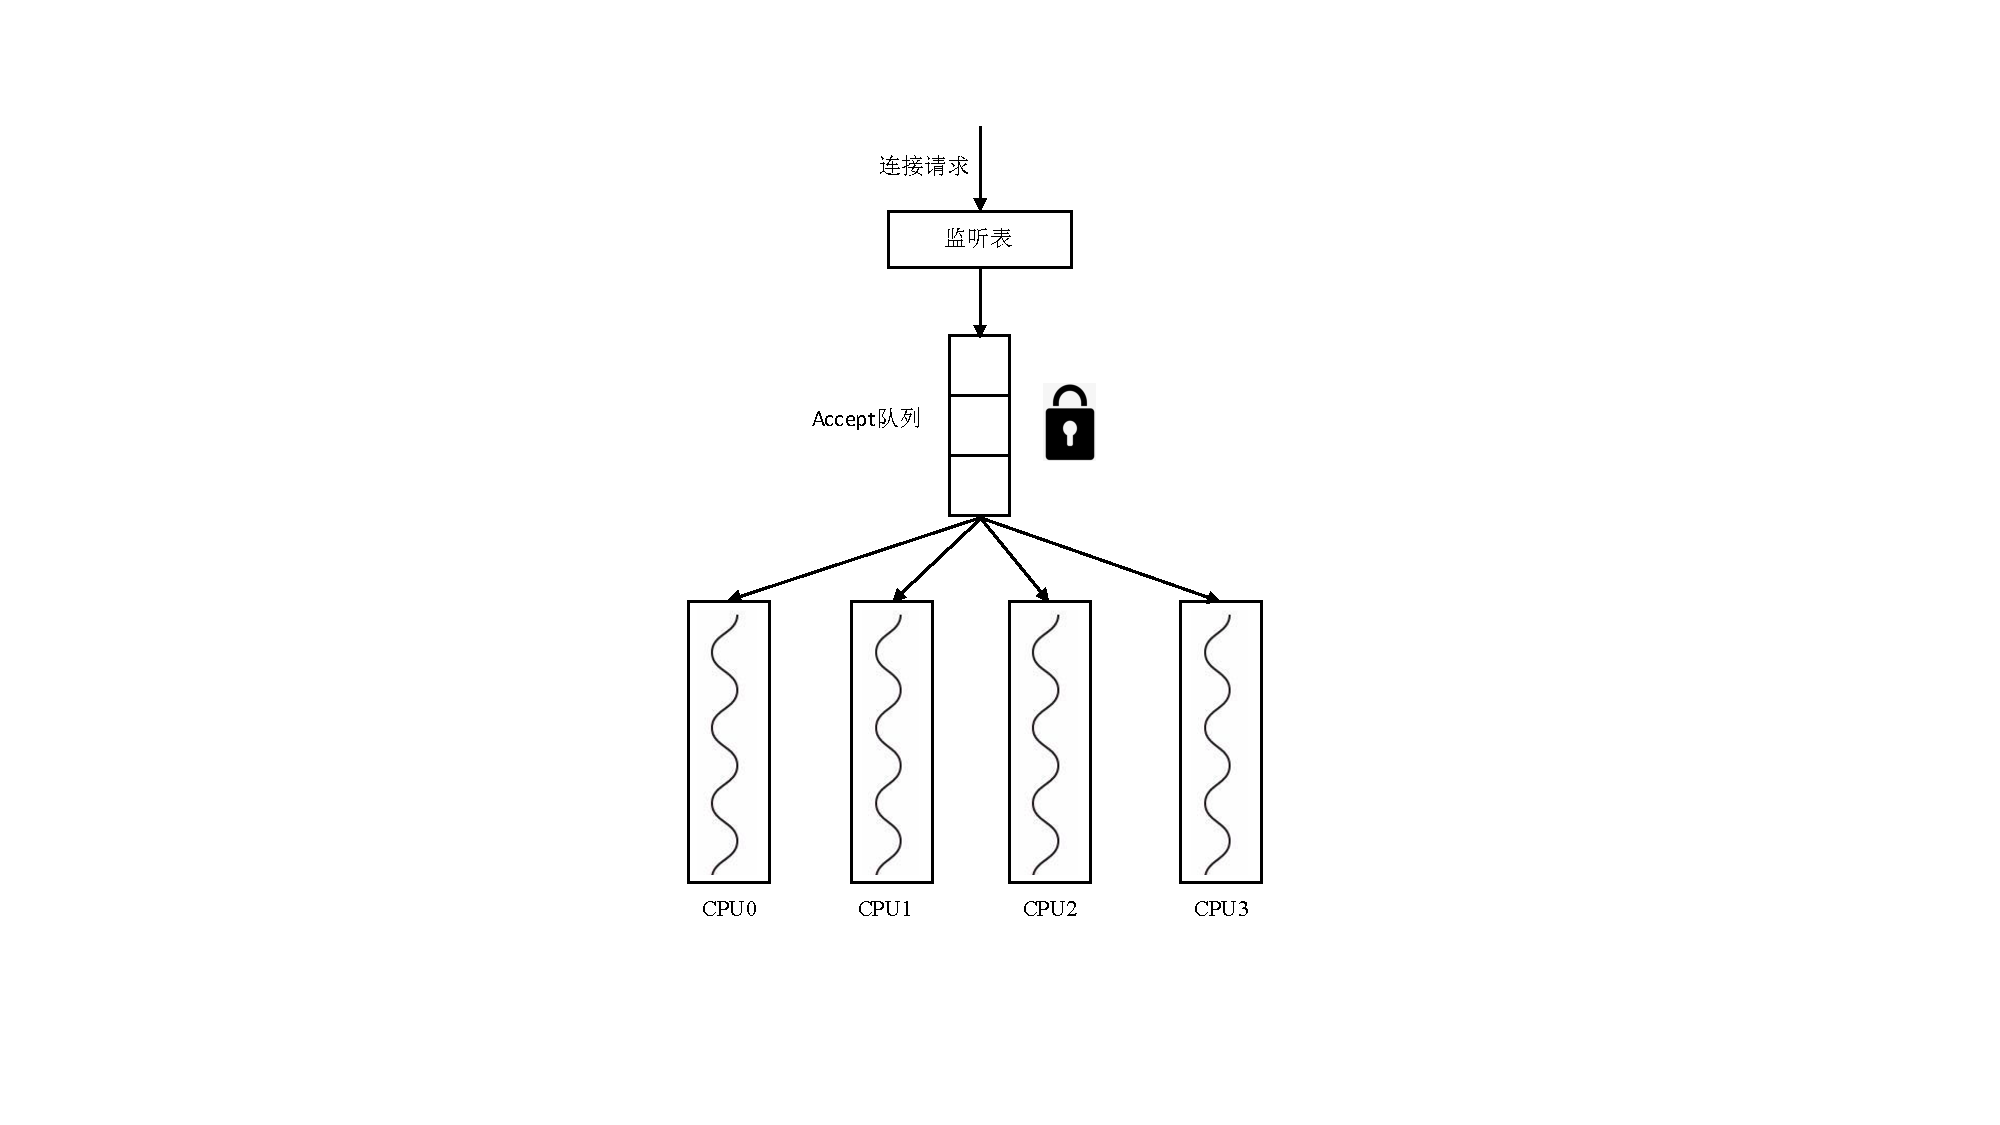
\includegraphics[width=6cm]{accept_queue_lock.pdf}
\caption{SO\_REUSEPORT引入之前}
\label{fig:accept_queue_lock}
\end{minipage}
\begin{minipage}[t]{0.48\textwidth}
\centering
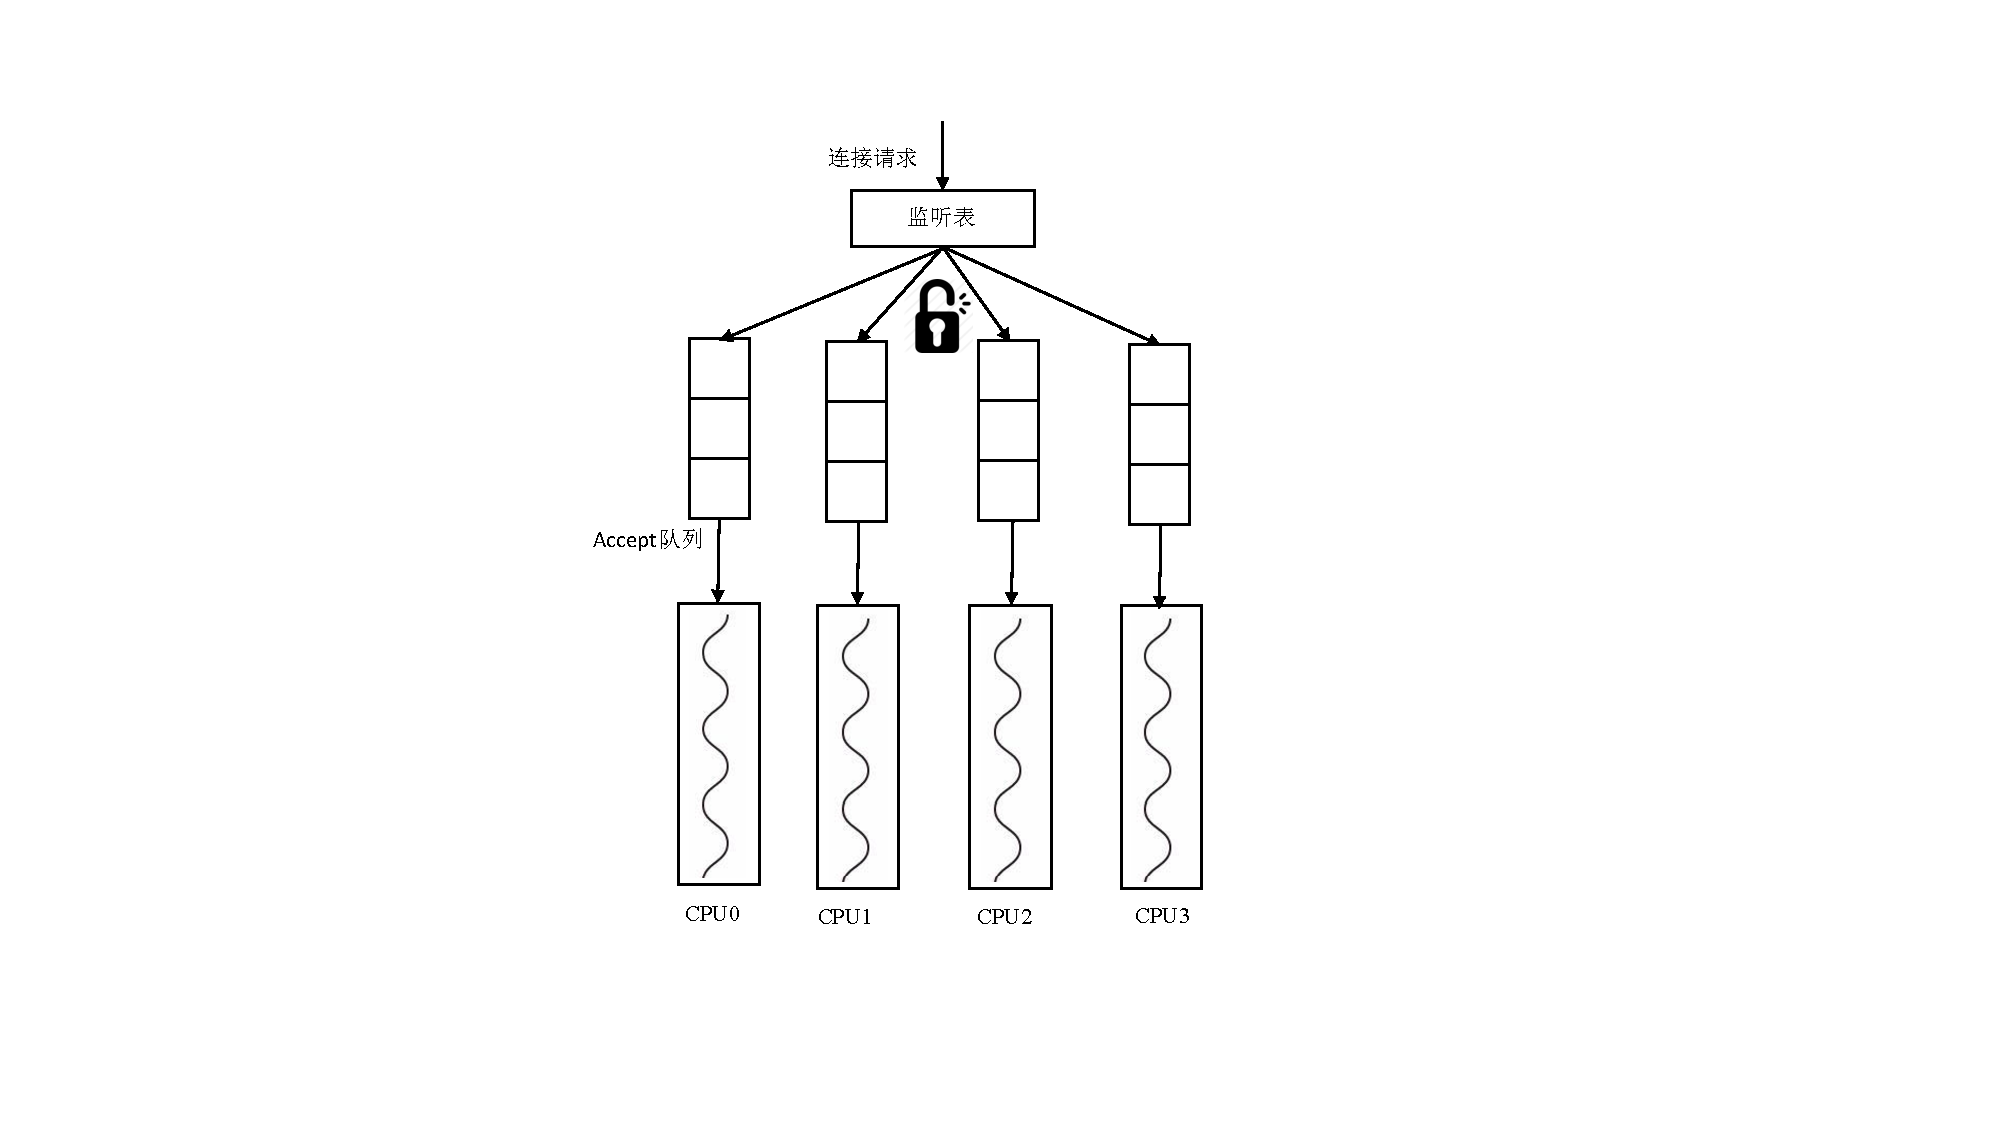
\includegraphics[width=6cm]{accept_queue_unlock.pdf}
\caption{SO\_REUSEPORT引入之后}
\label{fig:accept_queue_unlock}
\end{minipage}
\end{figure}
% \vspace{-10pt}

对于使用IO多路并发的服务器,比如Nginx中使用epoll,当多个并发流监听同一个listen socket存在着惊群现象,即多个执行流均在调用epoll\_wait函数发生阻塞,当一个新网络连接到达时,内核会唤醒所有执行流,但只有其中一个能真正接收该连接并进行数据传递,这在网络吞吐并不高的环境下无效的唤醒造成CPU等资源的浪费。Linux4.5版本中引入EPOLLEXCLUSIVE选项~\cite{EPOLLEXCLUSIVE}解决了Epoll惊群问题,但同样需要在调用epoll\_ctl函数时候添加该选项才能生效,对用户的兼容性也并不友好。
对网络协议栈中数据拷贝的优化在内核中也不断发展,sendfile是通过网络向远端发送本地磁盘文件的接口,它的出现减少了内核态与用户态之间的两次数据拷贝,但是由于该接口仅能应用于文件,并不支持socket之间的网络通信,对网络性能的提升有限,此外它并不属于POSIX或其他任何标准中,在各个操作系统中实现并不统一。在Linux4.14版本中采纳MSG\_ZEROCOPY~\cite{msg_zerocopy}选项来实现数据的零拷贝,该实现是基于虚拟化技术tuntap~\cite{tuntap}、vhost和xen~\cite{Xen}的零拷贝框架。然而该功能的生效既需要调用setsockopt函数为该socket设置SOCK\_ZEROCOPY选项,还需要在接收或发送的函数参数中加入MSG\_ZEROCOPY,应用兼容性更加不好。

从上面的介绍可以看出,操作系统内核对协议栈的优化虽然没有改变POSIX API本身,但还是需要用户修改网络应用源码,并且对网络性能的提升幅度有限。而发展缓慢的内核已经跟不上互联网流量膨胀的速度,于是大量从内核态对协议栈进行深度调优的工作不断涌现出来。

\subsection{内核态调优网络协议栈}

传统的网络协议栈无法保证在一个TCP连接整个过程,包括接收数据、内核TCP状态机处理、用户态代码执行、内存分配、发送数据这些阶段都只在一个核上进行,例如图5所示,数据接收以及三次握手建连的逻辑由CPU0来完成,但发送数据时候却由CPU2进行,在这种情况下跨核Cache数据的迁移造成CPU中Cache和TLB的Miss概率提升进而影响协议栈的整体性能。为了解决该问题,Affinity-Accept~\cite{Affinity-Accept}基于2.6.35版本的Linux内核通过accept队列本地化、减小连接Hash映射表锁的粒度等优化保证一个TCP连接全过程只在一个CPU核进行,实验显示,该优化在单核中降低30\%的TCP协议栈处理时间并提升24\%的整体网络吞吐。由于该优化是直接在Linux内核中并且完好地保持POSIX网络API,所以该方案理论上具备高兼容性,只不过对网络系统的提升有限。

作为同年发表的研究成果,MegaPipe~\cite{MegaPipe}在内核态对协议栈进行更大规模的优化,这是由于在面向消息的应用中,比如HTTP、RPC、DB、Key-value Store中,要么一个TCP连接传递的数据量较少,要么TCP连接时间较短,这些网络流量对服务器CPU资源是隐形杀手,毕竟CPU cycle的时间不少浪费在TCP三次握手和四次挥手这些网络逻辑中。MegaPipe的主要优化点如下:

\begin{enumerate}[(1),labelsep=.5em, leftmargin = 0pt, itemindent = 3em]
\item 通过在内核网络API与网络应用之间建立系统调用批处理的channel以最大程度降低网络系统调用引发上下文切换带来的开销。
\item 对listen socket中accept队列与hash建连表等资源进行本地化处理,与Affinity-Accept中优化相似。
\item 将虚拟文件系统VFS从网络socket中剔除,设计出更轻量级的socket API。
\end{enumerate}

文章实验结果显示这些优化与原内核网络协议栈相比在memcached中带来超过15\%的性能提升以及在Nginx中带来75\%左右的性能提升。然而,MegaPipe并不具备任何兼容性,因为其设计一套完全不同于原POSIX网络API的接口使其难以应用到众多网络应用中,再加上其并没有将源代码开源,也就使得它最终停留在实验室阶段。

socket接口中系统调用开销在另一篇文章~\cite{hruby2014sockets}得到更全面的分析,由于用户态陷入到内核态涉及到的安全权限的切换以及对CPU Cache、分支预测器、TLB等资源的污染,系统调用的开销也是不容忽视。尤其针对read、write、accept、select等这些在一次TCP连接中会被反复调用的接口,与MegaPipe重新设计网络API的策略相反,该文章通过将socket缓存暴露到网络应用等手段使得在网络高负载情况下消除99\%的系统调用开销,并将其用户加速基于微内核多服务器的系统NewtOS~\cite{hruby2012keep}。这种策略确实使其具备高度的兼容性,网络应用完全不需要修改源码即可运行在系统调用经过优化的POSIX网络接口上。然而该文章并没有明确阐述其与其他研究成果哪怕是Linux内核的性能对比。

Fastsocket~\cite{fastsocket,fastsocket-release}是最新对内核网络协议栈优化的研究成果,它在研究之初就是为了将系统最终落地到业界真实生产环境中,这就带来一些性能以外的考量,首先就是兼容性,包括网络API的兼容性、符合RFC规范、可以应用在主流常见网卡中,因为公司的网络服务众多,研发成本或硬件成本较大可能很难在公司中推广;此外还有协议栈的安全性,能抵御各种各样常见的网络攻击,如DDos拒绝服务攻击、连接劫持攻击等。

\vspace{-10pt}
\begin{figure}[H] % use float package if you want it here
  \centering
  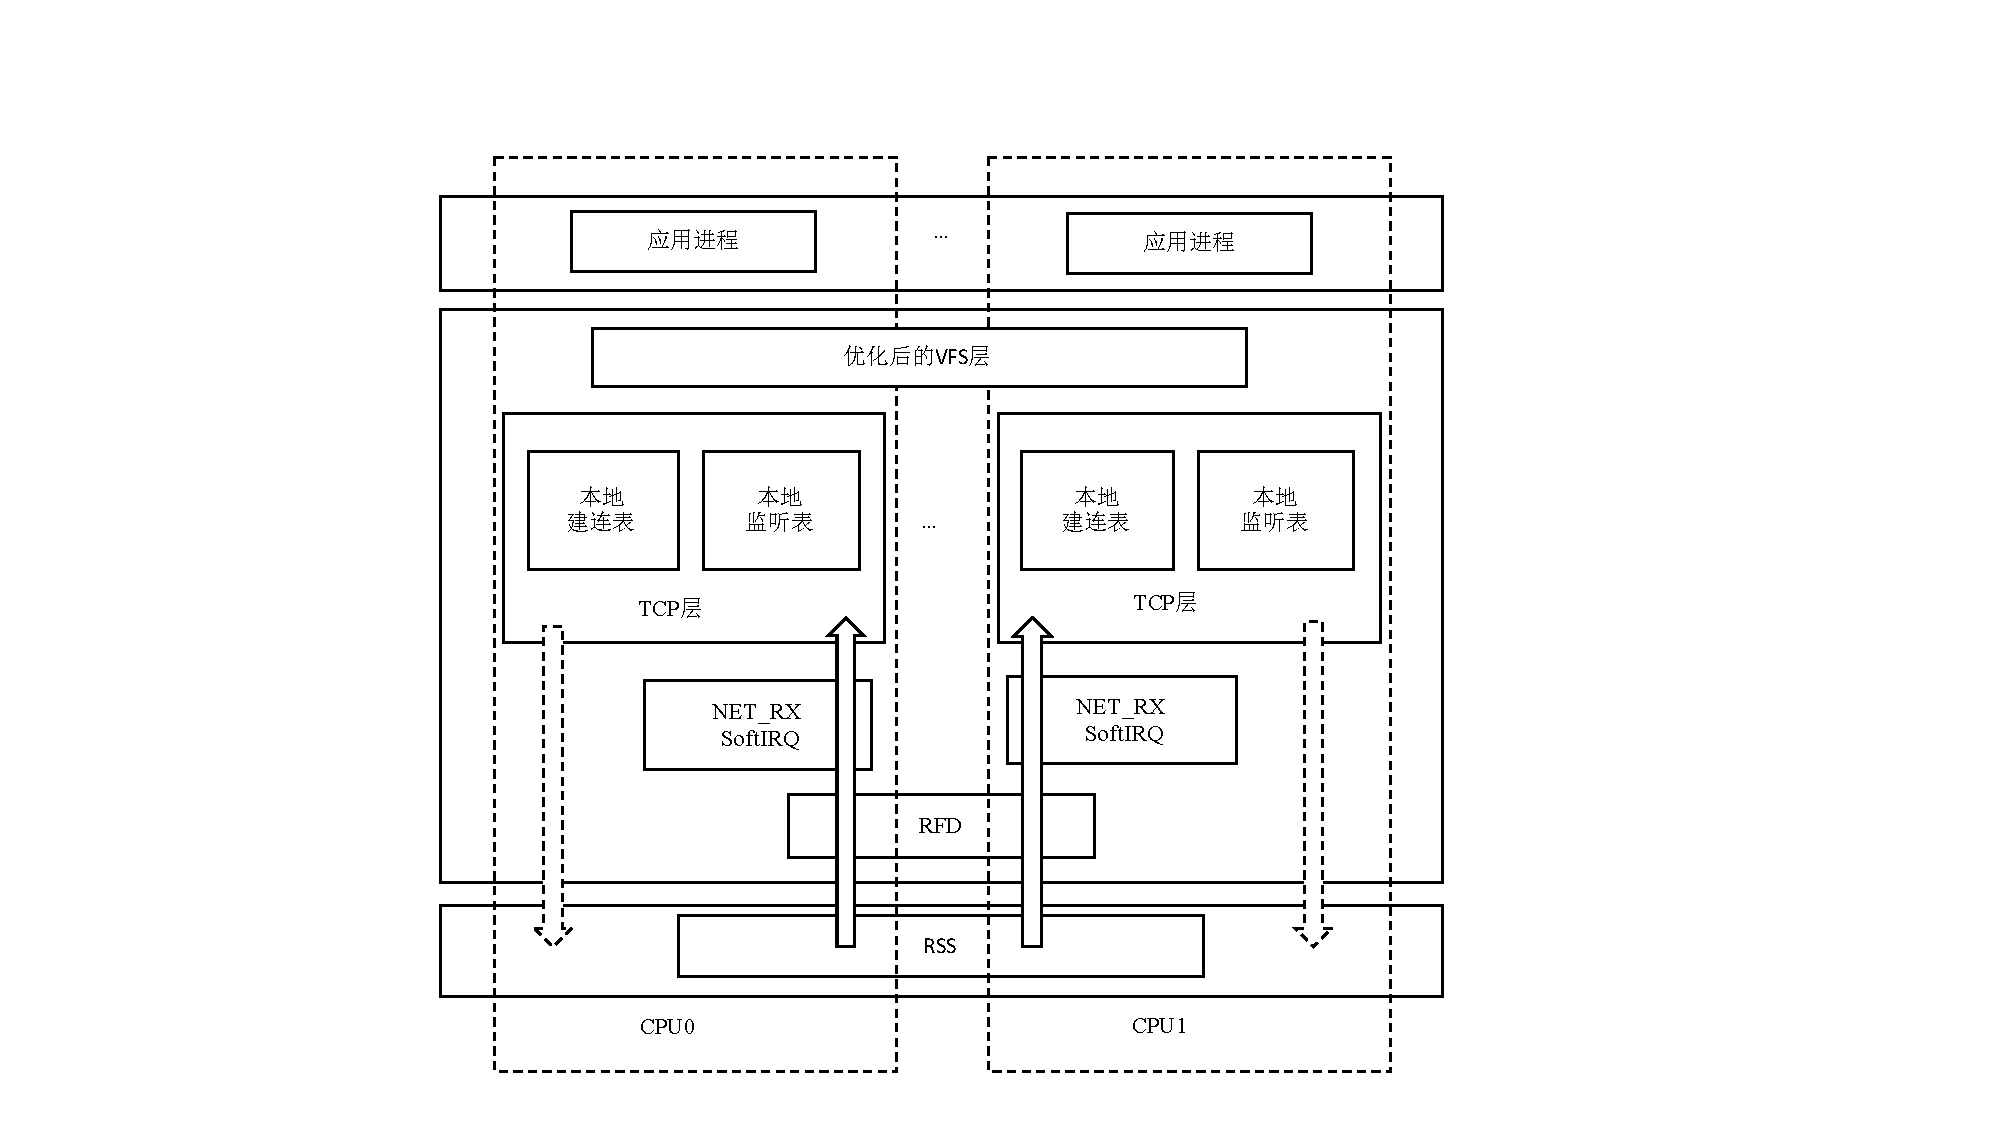
\includegraphics[width=\textwidth]{fastsocket}
  \caption{Fastsocket架构图}
  \label{fig:fastsocket}
\end{figure}
\vspace{-10pt}

基于以上的研究目的,Fastsocket在内核态对协议栈也是在TCP连接共享资源的拆分、虚拟文件系统VFS的优化、连接本地化这三方面进行更加彻底的优化。其系统架构图如图\ref{fig:fastsocket}所示,Fastsocket首先在底层通过RSS (Receive Side Scaling)和RFD(Receive Flow Deliver)来分别实现被动连接和主动连接的本地化,即网络服务不论是监听套接字接收连接还是调用connect函数发起连接,都可以保证整个TCP连接过程中仅发生在唯一一个CPU核上。被动连接直接根据网络请求的五元组计算CPU号来完成本地化,而对于更为复杂的主动连接,当网络服务调用connect主动发起连接 请求时,Fastsocket会依据该服务所在线程对应的CPU号计算出该网络连接的源端口号,而不是像传统内核一样随机产生,当该连接接收到对端的响应报文时候便根据该端口号逆向计算出对应的CPU号,之后就交给该CPU进行网络处理,如此反复进行,这样主动连接的整个TCP连接就都在唯一一个核上进行。连接本地化避免TCP数据在CPU之间跨核造成Cache、TLB Miss,从而提升了性能,此外它也为TCP建连表与监听表等资源按CPU级别拆分提供支持。Fastsocket中每一个core拥有自己独立的TCP建连表与监听表,一旦有新连接到来,通过RSS调度到某一CPU核后,协议栈会就会在该CPU 核运行一个内核线程来处理该连接,这样新建连接的TCP报文只需要在该CPU核中的建连表进行查询即可,避免并发流处理中锁同步竞争的开销,监听表也与此类似,也正是因为有连接本地化作为基础,不会存在后来的报文到达另外CPU核中而丢失TCP建连表信息的问题,这大大提升了协议栈的多核扩展性。



此外,Fastsocket也对VFS进行优化,因为据实验分析~\cite{boyd2010analysis},在流量负载较高且socket频繁申请的情况下,VFS花费不少时间去管理全局可见的inodes和dentries资源,去除socket在文件系统实现中inode\_lock这些对网络系统无关轻重的锁。实验结果显示Fastsocket在24核系统中实现了20.4倍相对于单核系统加速,多核扩展线性系数达到0.85,在Nginx和HAProxy网络应用中与Linux内核对比分别提升267\%和621\%之高。此外,更是因为其具备很好的兼容性,即不需要修改应用源码就可部署的低成本优势,使得其已经在新浪微博公司的真实生产环境中落地,从中不难看出兼容性对于网络协议栈能否真正被应用的重要性。

在内核中对协议栈进行优化在一定程度上可以保留Socket API,具备较好的兼容性,也能很好的解决原内核协议栈中多核扩展性的问题。不过由于数据在内核态与用户态的拷贝,传统基于中断的IO收发包模式的低效,难以完全避免的系统调用开销这种问题在内核态都难以得到解决,所以它带来的性能提升往往比较有限。此外,网络协议栈局限在内核中也会减缓其本身的发展速度,具有不方便调试等一系列问题。

\section{用户态优化网络协议栈}
\label{sec:userspace}
内核协议栈难以调试、发展受限等缺点在上个世纪八十年代就引起研究人员的注意,并不断尝试将协议栈搬离到用户态来实现,包括探索微内核网络架构~\cite{maeda1994protocol}、网络性能优化~\cite{thekkath1993implementing,basu1995user,edwards1995experiences}等,但都无法取得优于内核协议栈的网络性能。在当时上下文切换和跨进程间通信是实现用户协议栈两大性能障碍~\cite{1987packer},向各个网络应用进行packet demultiplex的任务如果放到进行用户态进程来做,相比于内核态实现就会造成过多次的上下文切换。究其根本原因,就是当时的技术背景还没有出现一种性能较高的绕过内核直接完成网络收发包的技术,这也是在用户态实现高性能网络协议栈的基础。


\subsection{绕过内核(Kernel Bypass)技术}
\label{subsec:02_dpdk}

Kernel Bypass最常见的实现方式是利用高速IO网络收发包框架,它们通常是经过一系列优化专为高吞吐网络流量环境设计。 IO虚拟化为协议栈网卡资源管理和绕过内核带来新的思路。SR-IOV为多虚拟机系统的高速IO共享同一物理网卡资源提供规范,一个带有SR-IOV~\cite{dong2012high}功能的物理网卡能被切分为多个独立的功能子模块,每一个功能模块都可以像一块独立的物理网卡为上层网络应用提供服务。Hypervisor软件去创建这些虚拟的功能模块,并在SR-IOV虚拟网卡中配置过滤规则去对数据包进行demultiplex,从而到达不同的网络协议栈。基于高速IO模块的网络应用性能通常要更好,但是会独占网卡使其无法收发内核协议栈数据包,而IO虚拟化可以与内核协议栈的网络通信共享同一物理网卡资源。此外,Rump Kernels~\cite{kantee2014rump}、User Mode Linux~\cite{dike2001user}也可以用来绕过内核直接在用户态运行应用,不过这些并不是针对网络协议栈设计,此文不予赘述。下面重点针对高速IO收发包模块这个在用户态协议栈中常用的技术进行展开介绍。
DPDK~\cite{DPDK}是Intel公司推出的一款高速处理数据包的框架,基于DPDK提供的包括收发包、定时器、内存管理等全套组件,网络应用可以完全与内核操作系统解耦来实现网络性能提升。根据其官网实验结果显示,在纯二层转发测试下,DPDK处理一个数据包仅需要80个CPU时钟周期,而CPU进行一次DRAM主存访问还需要上百个CPU周期。如此高的性能得益于如下几点优化:

\begin{enumerate}[(1),labelsep=.5em, leftmargin = 0pt, itemindent = 3em]
\item 大页内存管理其数据结构,其大小通常从2MB到数GB可灵活配置,而操作系统默认的内存页大小是4KB,这样可以大大减少TLB缓存Miss几率和缺页中断的发生。
\item 使用轮询替代中断的IO模式,在网络高负载情况下,中断收包模式下对CPU产生的硬件中断开销较大,轮询可以有效避免大流量时候频繁中断的开销。
\item 利用UIO网卡驱动实现Kernel Bypass,接收到的数据包直接可以在用户态进行处理,减少系统调用和数据包在内核态与用户态之间拷贝的性能开销。
\item RSS技术与亲核性机制将应用绑定在专门的CPU核中,减少数据跨核、Cache Miss带来的开销。此外,DPDK还利用CAS操作实现了一套无锁数据结构,例如rte\_ring等,这也减少锁带来的同步竞争开销。
\end{enumerate}

PF\_RING ZC (Zero Copy)~\cite{PF_RING}是在收发端均可实现1/10Gb线速转发的网络开发模块,当开启PF\_RING-aware driver时可以用来实现Kernel Bypass,从而减少系统调用开销。同时,PF\_RING ZC与其之前的版本都采用了内存预分配机制,并利用环形队列来实现内存资源的可重复利用,此外PF-RING ZC将用户态内存空间的地址映射到驱动的内存空间使得网络应用可以通过其API直接访问网卡的寄存器和内存数据从而实现了真正的零拷贝,然而这也为应用PF\_RING ZC编写网络应用程序带来因误操作网卡内存造成系统崩溃的安全隐患。

Netmap~\cite{NetMap}是一个高效的网络包处理模块,它通过数据包memory资源预分配减少每个数据包带来的内存分配的开销,利用网卡驱动buffer到用户态的内存映射技术实现零拷贝。Netmap的设计理念如图~\ref{fig:netmap}所示,当网络应用使用其接口接收数据时,网卡就与内核协议栈部分分离,使得数据可以绕过内核在共享内存中在网卡与应用之间进行传递,而对于传统操作系统的控制channel完全透明,OS的接口用来进行同步。所以严格来讲,Netmap在数据层面进行Kernel Bypass,而在控制层面依然依赖传统内核操作系统来完成信息传递。

高速IO收发包模块直接从网卡获得到二层数据裸包,在防火墙、流量监控等企业级服务器应用中使用较为方便,但要运行基于POSIX socket接口的网络应用,还需要独立的用户态网络协议栈对TCP/IP各层的网络逻辑进行实现。

\vspace{-10pt}
\begin{figure}[H] % use float package if you want it here
  \centering
  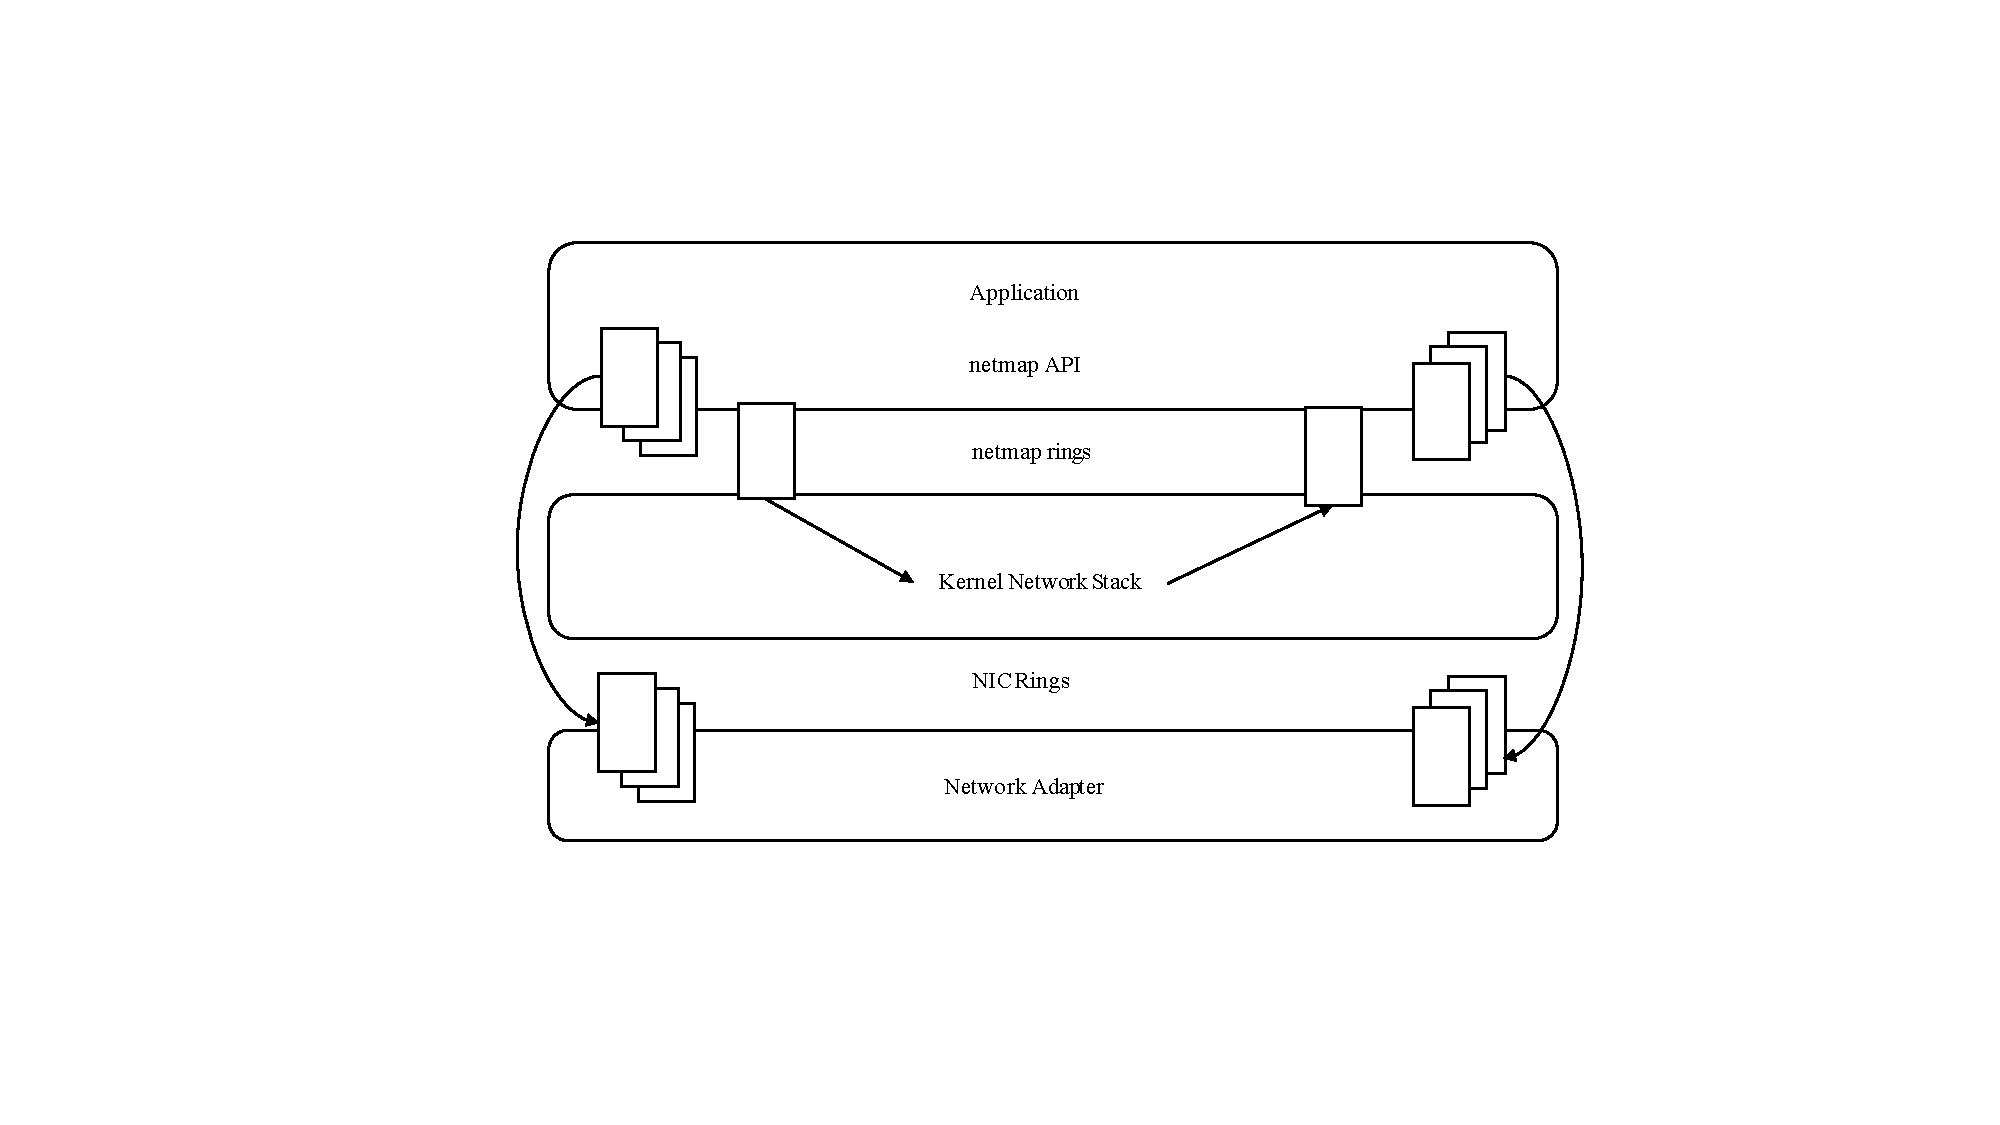
\includegraphics[width=\textwidth]{netmap}
  \caption{Netmap架构图}
  \label{fig:netmap}
\end{figure}
\vspace{-10pt}

\subsection{用户态协议栈的相关研究工作}
\label{subsec:02_userspace_related_work}

在具备高效的Kernel Bypass技术后,用户态协议栈最近几年在工业界和学术界都得到飞速发展。网络协议栈在用户态的实现可以选择两条路径,第一条是独立开发功能精简、定制化的协议栈,这样带来的网络性能提升更为可观,在定制化的场景下更具优化,然而往往缺失传统协议栈的安全性和鲁棒性;另一条路径是从传统内核协议栈中剥离出网络功能部分的代码,这需要在对熟练掌握内核协议栈实现的基础上去划分网络功能的边界,并用高速IO收发包模块的底层开发套件替换掉内核协议栈中网卡netdev、内存管理、定时器等边界函数实现,技术挑战较大,在兼顾高性能的同时可以保障系统的安全性与鲁棒性

mTCP~\cite{mTCP}是近些年学术界影响力很大并且已经开源的用户态协议栈,除了连接本地化、共享资源拆分等常见协议栈优化之外,mTCP从底层IO收包到用户态网络API都采用批处理操作,并且针对短连接进行基于优先级队列的报文处理优化策略,旨在提升短连接网络下多核系统的性能及可扩展性。其系统架构图如图~\ref{fig:mTCP}所示,底层用户态高速网络收包模块采用模块化的设计,可灵活支持PSIO、DPDK、netmap等模块,每一个CPU核拥有独立专享的TCP监听表、建连表等资源,避免锁竞争同步开销,且网络应用进程绑定在一个CPU核上,并含有一个mTCP协议栈线程执和一个网络应用线程,前者负责网络数据包的收发以及TCP/IP网络协议逻辑处理,后者负责网络应用代码执行逻辑,两者通过队列来完成线程间消息传递通信。
\vspace{-10pt}
\begin{figure}[H] % use float package if you want it here
  \centering
  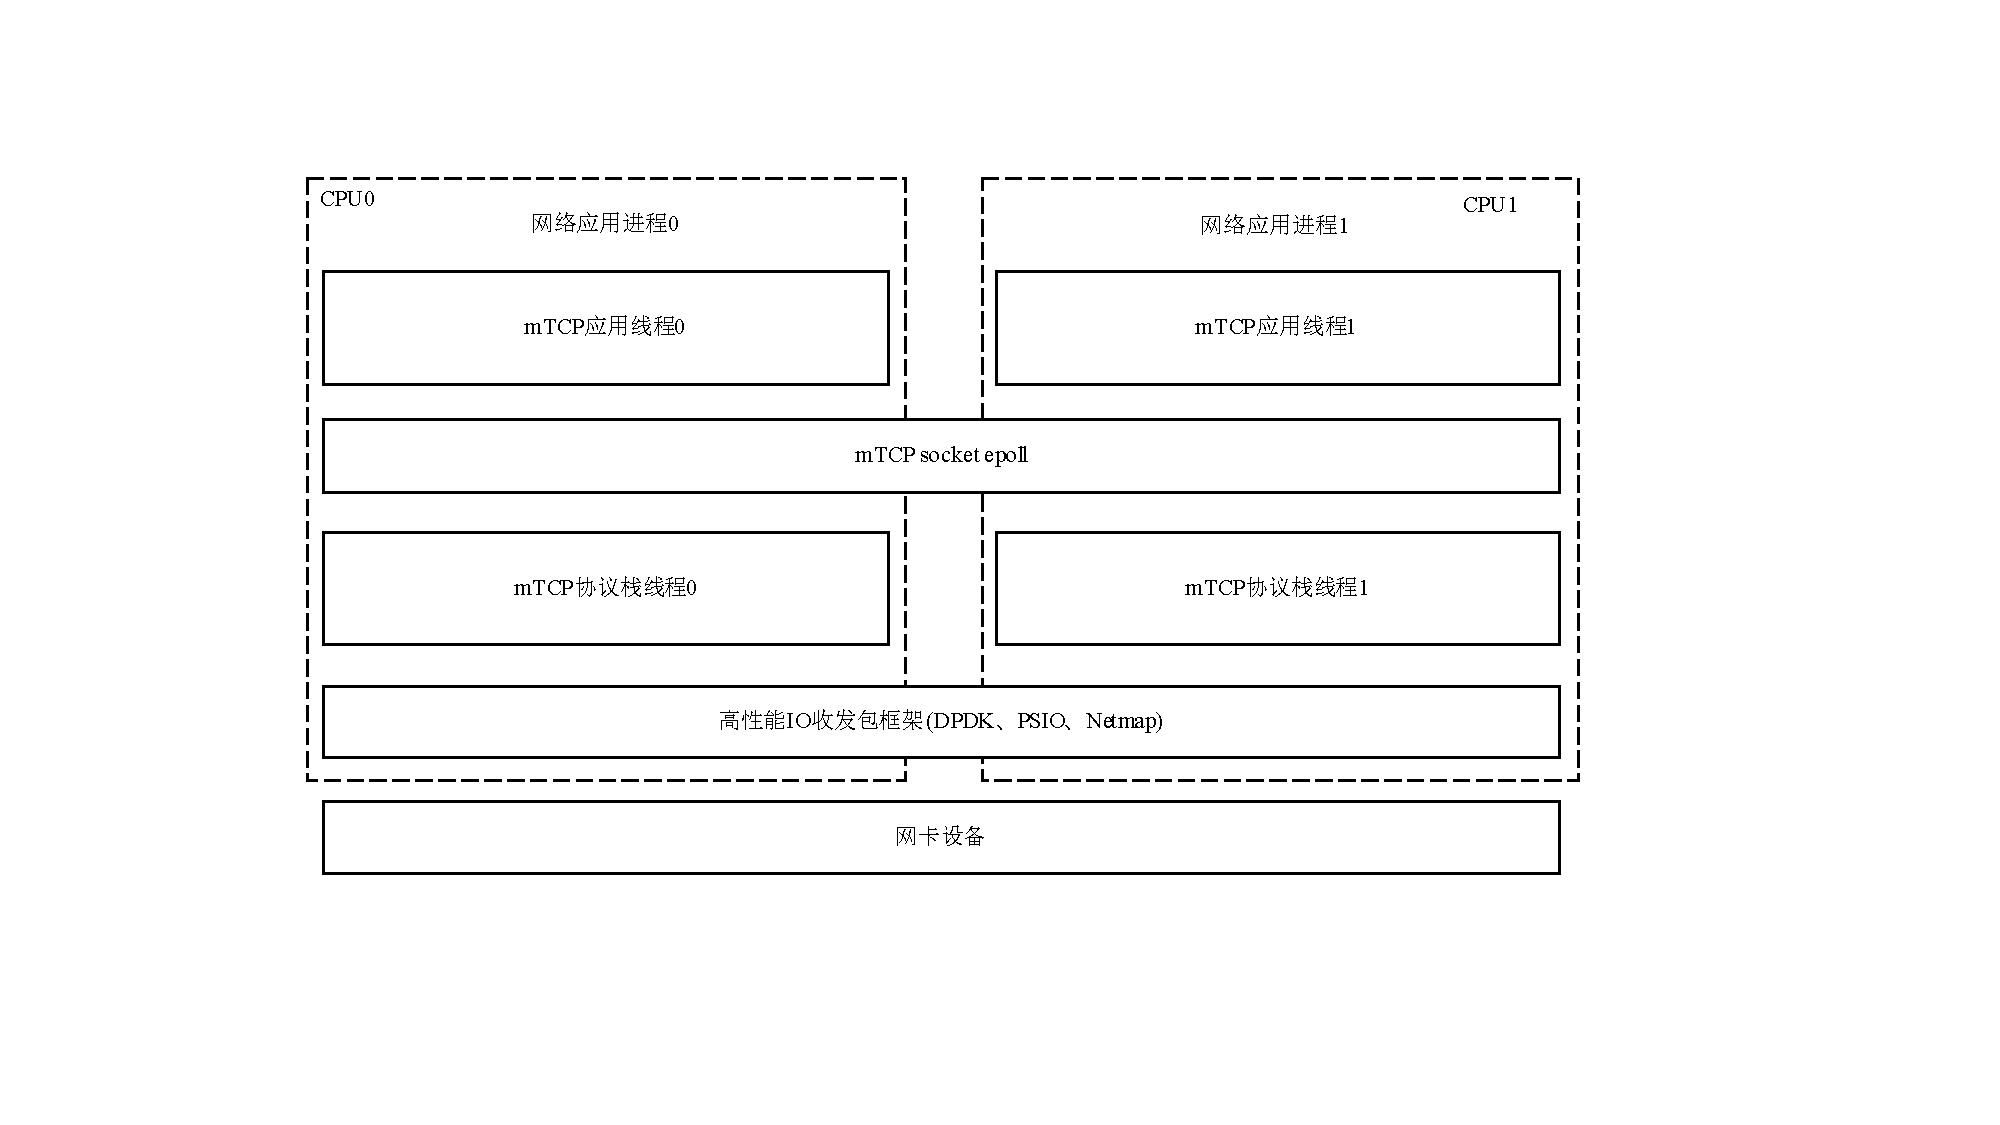
\includegraphics[width=\textwidth]{mTCP}
  \caption{mTCP架构图}
  \label{fig:mTCP}
\end{figure}
\vspace{-10pt}
不过,两个线程在同一CPU核上可能存在着严重的CPU资源争抢问题,在阅读其源码后了解到,mTCP是通过pthread条件变量来完成两个线程的调度,例如当mTCP线程完成一轮数据包的接收后产生新建连接、数据包接收等多个event,并将其放入event队列后,便会调用pthread\_cond\_signal去唤醒网络应用线程在epoll\_wait函数阻塞的执行流,而mTCP线程将会被挂起。mTCP通过这种主动让出CPU的调度策略最大程度上利用一个CPU核资源,但同时不可避免导致线程上下文切换带来的开销,mTCP是通过对接收报文、event通知的批处理操作来最大程度均摊上下文切换的开销,并且实验结果显示,mTCP在8核系统中相比于传统Linux网络协议栈带来25倍性能的提升。
然而mTCP正如其名是一个独立开发且只支持TCP传输层协议栈的网络协议栈,基于UDP的网络应用是无法应用于其上,并且其epoll接口未对非socket类型文件描述符进行支持,因为不少应用存在着用epoll对文件、管道等资源进行监控的情况,所以mTCP并不能支持这类网络应用的运行。此外,mTCP向上暴露的接口是类似POSIX API,虽然文章中指出只需要对网络应用进行少量源码修改即可,但从其开源至今四年多时间里,mTCP也仅支持了Lighttpd这个较为主流的网络应用服务器,有不少开发人员对Nginx进行移植尝试~\cite{nginxmtcp1,nginxmtcp2},但经过实验验证,均无法正常运行或者性能不及Linux内核协议栈。这也说明即使一款开源且性能优异的用户态协议栈在不具备高兼容性的情况下,其影响力也会大打折扣。

Sandstorm~\cite{Sandstorm}指出传统协议栈由于通用性带来性能瓶颈,并呼吁协议栈在数据中心这种低延迟高吞吐的网络环境下应该往专用性方向发展。然而该文章依然利用netmap作为底层IO收发包模块来减少数据拷贝,并将协议栈搬离到用户态来实现,在用户态优化协议栈的手段并未有任何创新,实验结果使用移植Nginx作为网络服务相比传统Linux内核协议栈有三倍左右的性能提升,但是其在测试SandStorm性能时将静态文件缓存到物理内存中,这与Linux内核协议栈的Nginx从磁盘中读取文件直接对比未免有失公平,这样的性能提升在兼顾通用性的用户态协议栈也能做到。所以,性能瓶颈的本质并不一定缘于协议栈的通用性或者兼容性,而是应该着眼于数据拷贝、进程间通信、系统调用、上下文切换等这些在网络协议栈中真正影响网络性能的关键。


MultiStack~\cite{Honda2014Rekindling}与StackMap~\cite{StackMap}是在用户态协议栈与兼容传统网络应用之间而采取折中策略。两者的核心思想都是将用户态协议栈与传统内核协议栈进行整合,MutiStack具体实现上最底层使用IO虚拟化技术进行Packet Demultiplex,向上承载着用户态协议栈和内核协议栈两种系统,用户态路径对应的虚拟网卡使用netmap作为收发包框架,内核态路径对应的虚拟网卡使用传统基于中断的收包模式。StackMap在设计上采用数据通道和控制通道分离的思想,数据通道通过netmap高性能收发包模块来减少数据拷贝,并向上层应用提供新型收发包API,而控制通道依然走传统内核协议栈来完成。这类折中设计只是让整个系统既可以运行传统网络应用,又能运行高性能新网络应用,不过,当下虚拟化技术非常成熟,创建一个新的虚拟机便捷又快速,这样整合的设计的意义并不大,而且其并没有解决兼容性的问题,因为网络应用若想获得用户态协议栈带来的加速依然需要根据新API语义进行重新编写。

IX~\cite{IX}采用数据平面与控制平面分离的策略,控制平面负责对CPU和内存资源配置、申请、调度和监控,数据平面负责网络协议栈的逻辑处理,并利用IO虚拟化技术将数据平面不同网络应用进行隔离,以保证安全性。IX数据平面的收包是在特定网卡上基于轮询IO模式进行的,这样可以减轻中断收包模式在大流量网络情况下由于硬件中断对CPU造成的压力。除了常见的协议栈优化策略,如图~\ref{fig:IX}展示一个IX中线程采用Run-to-Completion的工作模式,从虚拟网卡接收一个数据包,到协议栈网络逻辑处理,到交付给网络应用再到应用返回响应数据,经过协议栈后最终到达网卡进行发包,整个过程处理完才进行下一个数据包的处理,这样带来的好处是减少系统中不必要的缓存队列从而最大化降低网络延迟。当出现网络拥塞的情况,IX会对收发包和系统调用进行动态调整的批处理,以均摊上下文切换带来的开销。

\vspace{-10pt}
\begin{figure}[H] % use float package if you want it here
  \centering
  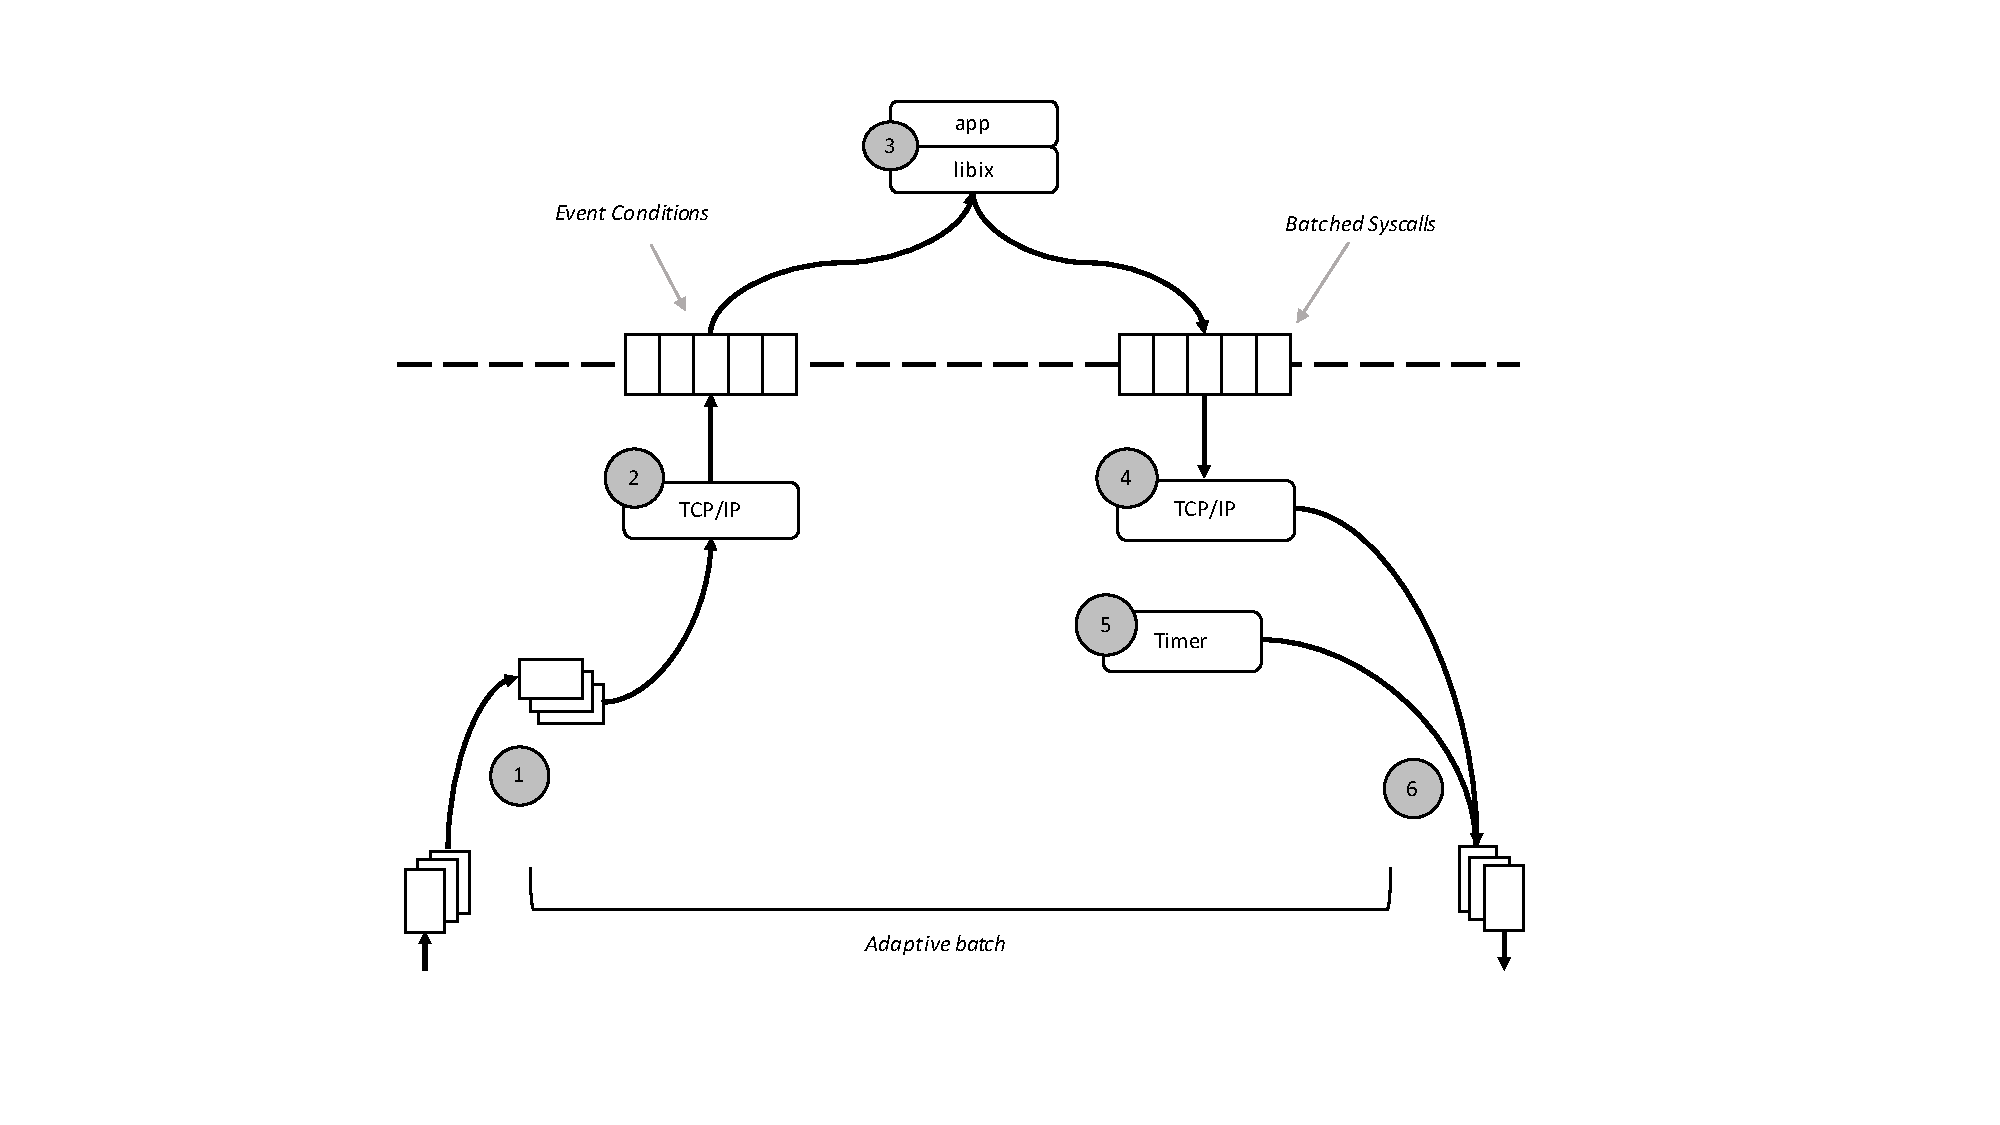
\includegraphics[width=\textwidth]{IX}
  \caption{IX Run-to-Completion工作模式}
  \label{fig:IX}
\end{figure}
\vspace{-10pt}

ZygOS~\cite{ZygOS}致力于解决网络执行流在不同核之间的调度问题而实现微秒级延迟和满足超低尾延迟要求,相比IX性能更加优秀,但两者都对网络应用毫无兼容性考虑。Arrakis~\cite{Peter2015Arrakis}也是采取将数据平面从内核中剥离的策略和IO虚拟化技术和内存映射等机制,并基于轻量级网络协议栈lwIP~\cite{lwIP}。不过该文章在兼容性方面做了更多考虑,Arrakis给网络应用暴露Native Arrakis API和POSIX API两种,前者由于重新设计数据IO的接口而实现真正的零拷贝,后者由于POSIX API 中recv 、send收发函数中带有应用buffer的语义无法实现真正的零拷贝,但也取得相比传统内核协议栈性能上的提升。

工业界近几年也开发出多款用户态协议栈~\cite{libuinet,pope2011introduction,Seastar,fstack}去加速公司网络服务性能,其中腾讯云推出的F-stack~\cite{fstack}基于DPDK高速IO收发包框架并移植FreeBSD网络协议栈来实现加速网络服务,并已经在DNS服务器、CDN接入模块等实际生产环境中落地,不过其接口是POSIX-Like,需要网络应用修改相应网络接口才能应用。Seastar~\cite{Seastar}是基于事件驱动、纯异步编程且用C++实现的用户态协议栈,其兼容性很差,因为接口是完全不同于Socket编程接口,且需要掌握更为复杂的异步编程模型。